%
% ---------------------------------------------------
%
% Trabajo de Final de Grado:
% Author: Gonzalo Jesús García Martín <dracoyue@gmail.com>
% Capítulo: Introducción
% Fichero: Cap1_Introduccion.tex
%
% ----------------------------------------------------
%

\cleardoublepage
\chapter{Introducción}
\label{chap:intorduction}

%¿Cúal es el tema del trabajo? ¿Por qué se hace el trabajo?
\CollegeApp persigue\cite{prueba:online} crear un sistema con el que los padres y sus hijos se puedan comunicar con los profesores de forma continua empleando las --ya no tan-- nuevas tecnologías. Esta temática surge a partir de los problemas escolares que se han ocasionado en los últimos años, como el acoso escolar o la falta de comunicación del personal docente con los padres y alumnos.

\bigskip
%¿Como está pensado el trabajo? ¿Cúales son las limitaciones del trabajo?
La aplicación se convierte en una herramienta para que los profesores puedan transmitir continuamente toda la información que ellos consideren relevante a los padres de sus alumnos. Esto evitará sorpresas desagradables, malentendidos e incluso algunos problemas.
Pero siempre estará limitado a la como se comuniquen los usuarios, ya que no se puede controlar el uso que éstos le den.

\section{Tecnologías}
	Las tecnologías usadas son las siguientes:
	\begin{itemize}
		\item {\bf AndroidStudio}\cite{1:androidstudio:online}: IDE\cite{12:ide:online} oficial para el desarrollo de aplicaciones para Android, basado en IntelliJ IDEA \cite{3:intellij:online}.
		\item {\bf Android}\cite{2:android:online}: Sistema operativo basado en el núcleo de Linux \cite{4:nucleolinux:online} para dispositivos móviles, televisores, automóviles y relojes inteligentes \cite{5:wearables:online}.
		\item {\bf Firebase}\cite{6:firebase:online}: Web que proporciona servicios en la nube de forma fácil y segura, con una integración bastante sencilla con las nuevas tecnologías. Ofrece servicios de recuperación y guardado de datos, registro y acceso de usuarios, reglas de seguridad, simulador y análisis de datos entre otros. Los datos almacenado en este servicio no son datos \href{http://es.wikipedia.org/wiki/SQL}{\textit{SQL}}\cite{8:jquery:online}\cite{9:jquery:online}, si no que son datos \href{http://es.wikipedia.org/wiki/JSON}{\textit{JSON}}\cite{7:json:online}. Sistemas con los que está integrado:
		\begin{itemize}
			\item {\bf Android}\cite{2:android:online}.
			\item {\bf IOS}\cite{10:ios:online}: Sistema operativo para dispositivos móviles propiedad de Apple Inc.
			\item {\bf Servicios Web}.
			\item {\bf Servicios REST}\cite{11:rest:online}.
		\end{itemize}
	\end{itemize}
	
	\subsection{Selección}
	%Por qué seleccionamos las herramientas seleccionadas
	A rellenar esta sub sección.
	
	\subsection{Otros IDE's: Eclipse}
	%Eclipse
	
	\subsubsection{Instalación de Eclipse}
	%Instalación de Eclipse
	
	\subsection{Otros Servicios en la Nube: Parse}
	%Parse
	
	\subsubsection{Instalación de Parse}
	%Uso de Parse
	
\section{Instalación}

	En esta sección se procederá a explicar la instalación de las herramientas usadas.

	\subsection{AndroidStudio}
		\begin{itemize}
			\item {\bf JDK}: Descargar e instalar {\it ``Java Development Kit''}\cite{17:jdk:online}.
			\item {\bf Descarga}: Descargar AndrodiStudio\cite{13:androidstudiodescarga:online}.
			\item {\bf Instalación}: Ejecutar el archivo de instalación descargado y seguir los pasos indicados por el instalador.
			\item {\bf SDK}: Añadir paquetes SDK con el gestor de paquetes ({\em ``SDK Manager''}) seleccionándolo en la barra de herramientas.
				\begin{figure}[h]
					\centering
					
\includegraphics{SdkManager}
					\caption{Icono SDK Manager}
					\label{fig:SdkManager}
				\end{figure}
			\item {\bf Paquetes}: Seleccionar las versiones de Android\cite{2:android:online} a instalar, se pueden elegir o quitar paquetes concretos de cada versión. Darle a {\em ``Install''}. Es importante que ademas de instalar las versiones a utilizar, se instalen los siguientes paquetes:
				\begin{itemize}
					\item Android SDK Tools.
					\item Android SDK Platform-tools.
					\item Android SDK Build-tools (La versión más actual).
					\item Extras \textgreater Android Support Repository.
					\item Extras \textgreater Android Support Library.
					\item Extras \textgreater Google USB Driver.
				\end{itemize}
		\end{itemize}
		
		\begin{figure}[h]
			%\noident
			\centering
			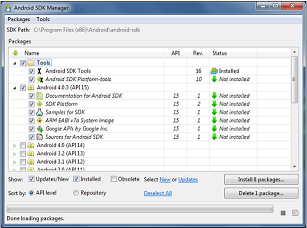
\includegraphics{Packages}
			\caption{Paquetes en SDK Manager}
			\label{fig:SdkManagerPackages}
		\end{figure}
		
	\newpage %Necesario para que la imagen aparezca antes de Firebase
	\subsection{Firebase}
		\begin{itemize}
			\item {\bf Librería}: Añadir la librería de Firebase en el archivo {\it ``build.gradle''} que esta dentro de la carpeta {\it ``app''} en el directorio del proyecto.
			\item {\bf Uso}: En los archivos de clase {\it ``java''}\cite{14:java:online} seguir los siguientes pasos:
				\begin{itemize}
					\item {\bf Cliente Firebase}: Importar la librería del cliente.
					\item {\bf Errores Firebase}: Importar la librería de errores en consultas.
					\item {\bf Datos Firebase}: Importar la librería que permite la devolución de datos desde Firebase.
					\item {\bf Consultas Firebase}: Importar la librería para consultas.
					\item {\bf Librería Oyentes}: Importar la librería de los oyentes ({\it ``Listeners''}).
					\item {\bf Contexto}: Añadir el contexto en que se va a usar en la función {\it onCreate}.
					\item {\bf Referencias}: Añadir una referencia a la base de datos o tabla de la misma a la que se van a hacer las consultas.
					\item {\bf Consultas}: Preparar la consulta que se va a hacer.
					\item {\bf Oyentes}:Añadir un oyente ({\it ``Listener''}) a la consulta.
				\end{itemize}
		\end{itemize}
		
		%Añadir codigo: Code/firebase.java
		\lstinputlisting[float,language=Java,caption={Ejemplo de uso de {\it Firebase}},label={code:firebase}]{Code/FirebaseExample.java}